\section{Pai}

26 juin 2008

\begin{multicols}{2}

Pai... petite ville encaissée dans les montagnes, au Nord Ouest de Chiang Mai, dans le triangle d'or de la drogue aux frontières du Myanmar, du Laos et de la Thaïlande. Pai a donc été mon étape suivant Chiang Mai. Je devais y retrouver là deux Québécois pour aller au Laos ensuite avec eux. Ce que j'avais pas vu c'est qu'en fait, ces deux jeunes frère et soeure sont du genre je dit un truc et je fais l'inverse. Du coup je les ai vite oubliés.

Durant les trois heures de bus pour Pai, j'ai rencontré Ammar, photographe et videaste Syrien. Nous avons passé une bonne partie des quatre jours ensemble.

\hspace*{-0.65cm}
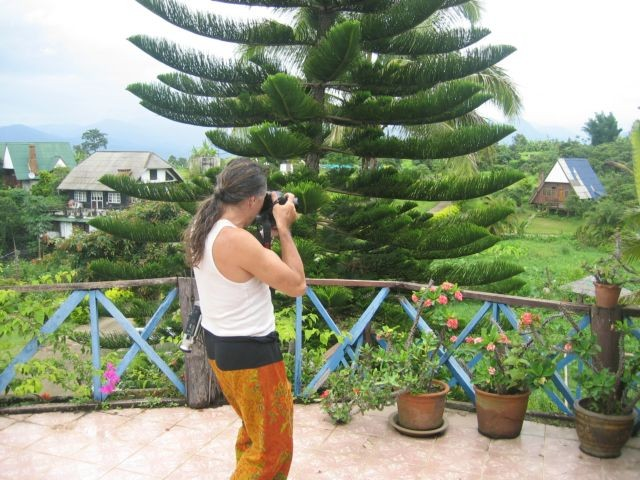
\includegraphics[width=4.8cm]{articles/Pai/1214286262syiV.jpg}
Ammar.

Nous avons là encore fait des tours en motor bike, pour se ballader, prendre des photos...

%<div><object width="640" height="505"><param name="movie" value="http://www.dailymotion.com/swf/x5x4t5&related=1"></param><param name="allowFullScreen" value="true"></param><param name="allowScriptAccess" value="always"></param><embed src="http://www.dailymotion.com/swf/x5x4t5&related=1" type="application/x-shockwave-flash" width="640" height="505" allowFullScreen="true" allowScriptAccess="always"></embed></object></div>

\hspace*{-0.65cm}
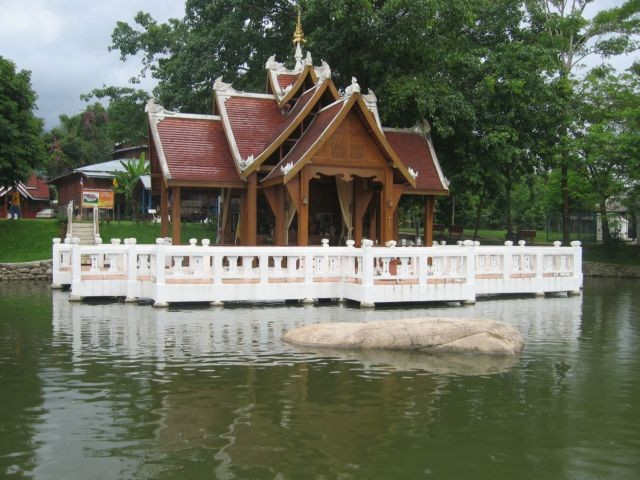
\includegraphics[width=4.8cm]{articles/Pai/1214286159uUtC.jpg}
Un petit temple, à moins que ce ne soit qu'un kiosque... ou p'têtre bien autre chose, allez savoir.

\hspace*{-0.65cm}
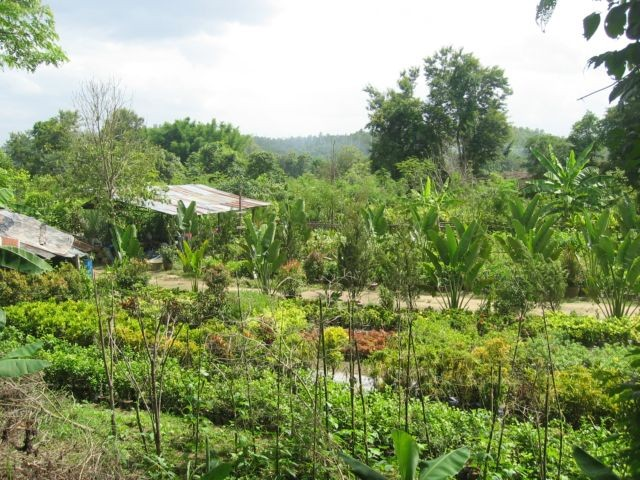
\includegraphics[width=4.8cm]{articles/Pai/1214286138yJBp.jpg}
La campagne autour de Pai.

Et regardez ce que l'on voit au detours d'un chemin : une guest house qui vous propose de dormir dans un arbre :

\hspace*{-0.65cm}
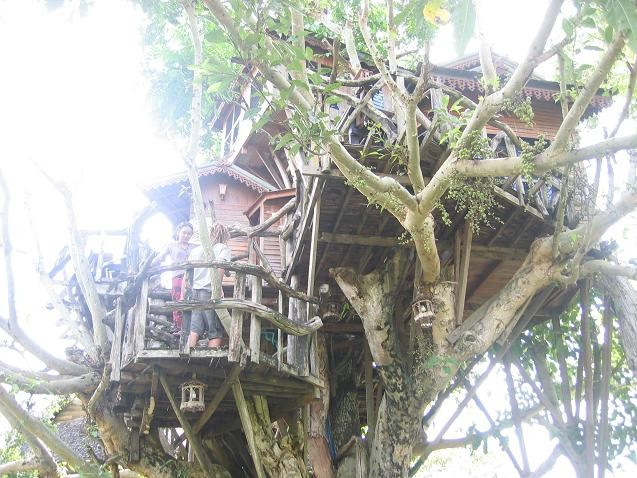
\includegraphics[width=4.8cm]{articles/Pai/1214471897bdDK.jpg}
Chambre originale.

Mais bon... la mienne c'est celle la :

\hspace*{-0.65cm}
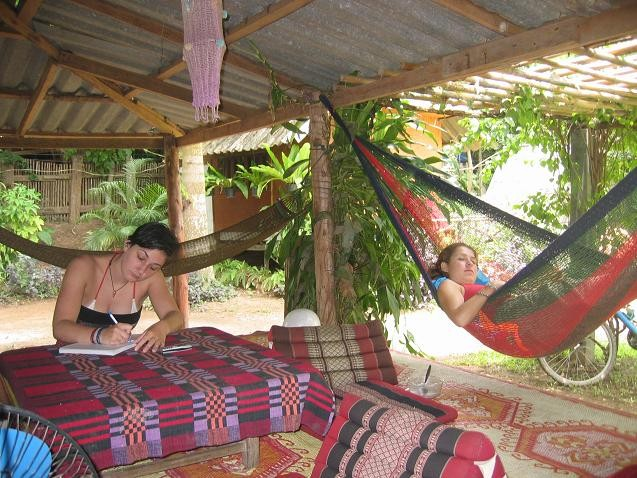
\includegraphics[width=4.8cm]{articles/Pai/1214471886LoCS.jpg}
Chill out.

J'en profite pour vous présenter Abby et Sue, deux Anglaise avec lesquelles on a passé un peu de temps aussi.

Revenez ici de temps en temps, des photos vont s'ajouter.

\end{multicols}

\bigskip
\textbf{\textsc{Commentaires}}

 \medskip
Titou a écrit le 26 juin 2008 :
\begin{displayquote}
On se demande vraiment pourquoi tu as choisi cette chambre .... :D pti veinard !
A plutch
\end{displayquote}


